%%%%%%%%%%%%%%%%%%%%%%%%%%%%%%%%%%%%%%%%%%%%%%%%%%%%%%
% A Beamer template for University of Wollongong     %
% Based on THU beamer theme                          %
% Author: Qiuyu Lu                                   %
% Date: July 2024                                    %
% LPPL Licensed.                                     %
%%%%%%%%%%%%%%%%%%%%%%%%%%%%%%%%%%%%%%%%%%%%%%%%%%%%%%
% Customized for Sharif University of Technology     %
%%%%%%%%%%%%%%%%%%%%%%%%%%%%%%%%%%%%%%%%%%%%%%%%%%%%%%


\documentclass[serif, aspectratio=169]{beamer}
%\documentclass[serif]{beamer}  % for 4:3 ratio
\usepackage[T1]{fontenc} 
\usepackage{fourier} % see "http://faq.ktug.org/wiki/uploads/MathFonts.pdf" for other options
\usepackage{hyperref}
\usepackage{latexsym,amsmath,xcolor,multicol,booktabs,calligra}
\usepackage{graphicx,pstricks,listings,stackengine}
\usepackage{lipsum}
\usepackage{tikz}
\usetikzlibrary{shapes.geometric} % Add this to include ellipse shapes
\usepackage{amsmath}
\usepackage{pgfplots}  % For plots
\usepackage{amsmath}   % For equations
\usepackage{array}     % For tables
\pgfplotsset{compat=1.16}

% \usetikzlibrary{positioning}


\author{Hooman Zolfaghari - Abdollah Zohrabi - Amirreza Velae}
\title{Neural Tangent Kernel}
\subtitle{Insights from High-Dimensional Probability}
\institute{
    Sharif University of Technology
}
%\date{\small \today}
% \usepackage{UoWstyle}
\usepackage{SUTstyle}

% defs
\def\cmd#1{\texttt{\color{red}\footnotesize $\backslash$#1}}
\def\env#1{\texttt{\color{blue}\footnotesize #1}}
\definecolor{deepblue}{rgb}{0,0,0.5}
\definecolor{deepred}{RGB}{153,0,0}
\definecolor{deepgreen}{rgb}{0,0.5,0}
\definecolor{halfgray}{gray}{0.55}

\lstset{
    basicstyle=\ttfamily\small,
    keywordstyle=\bfseries\color{deepblue},
    emphstyle=\ttfamily\color{deepred},    % Custom highlighting style
    stringstyle=\color{deepgreen},
    numbers=left,
    numberstyle=\small\color{halfgray},
    rulesepcolor=\color{red!20!green!20!blue!20},
    frame=shadowbox,
}

\begin{document}

\begin{frame}
    \titlepage
    \vspace*{-0.6cm}
    \begin{figure}[htpb]
        \begin{center}
            
\includegraphics[keepaspectratio, scale=0.25]{pic/sharif-main-logo.png}
        \end{center}
    \end{figure}
\end{frame}

\begin{frame}    
\tableofcontents[sectionstyle=show,
subsectionstyle=show/shaded/hide,
subsubsectionstyle=show/shaded/hide]
\end{frame}

% ============================ Introduction ============================ 
\section{Introduction}

\begin{frame}{NTK}
	
	The \textbf{Neural Tangent Kernel (NTK)} captures the behavior of fully-connected
	deep nets in the infinite-width limit trained by gradient descent. [Jacot et al., 2018]
	
	\begin{itemize}
		\item  An attraction is that a pure
		kernel-based method is used to capture the power of a fully-trained deep net of
		infinite width.
		
		
		\item NTK explains the evolution of neural networks during gradient descent training.
		\item Insight into why wide neural networks can consistently converge to a 
		global minimum when minimizing empirical loss.
	\end{itemize}
\end{frame}


\begin{frame}
\begin{itemize}
\item The convergence of kernel gradient descent to a critical point of the cost
C is guaranteed for positive definite kernels
\item In the case when the dataset is supported on a sphere, the
positive-definiteness of the limiting NTK can be shown
\end{itemize}
\end{frame}

\begin{frame}{Problem Definition}
	
	\begin{itemize}
		
		
		
		\item The NTK is defined using the gradient of the output of the randomly initialized net
		with respect to its parameters
		
		
		\item  At its core, it explains how updating the model parameters on one data sample affects the predictions for other samples.
	\end{itemize}
\end{frame}



\begin{frame}{Problem Definition}
	
	\begin{itemize}
		\item Model Parameters \(\theta \in \mathbb{R}^P\)
		
		\item The empirical loss function \(\mathcal{L}: \mathbb{R}^P \to \mathbb{R}_+\)
		to minimize during training is defined as follows, using a per-sample cost function \(\ell: \mathbb{R}^{n_0} \times \mathbb{R}^{n_L} \to \mathbb{R}_+\)
		\[
		\mathcal{L}(\theta) =\frac{1}{N} \sum_{i=1}^N \ell(f(\mathbf{x}^{(i)}; \theta), y^{(i)})
		\]
		\item  According to the chain rule. the gradient of the loss is:
		\[
		\nabla_\theta \mathcal{L}(\theta)= \frac{1}{N} \sum_{i=1}^N \underbrace{\nabla_\theta f(\mathbf{x}^{(i)}; \theta)}_{\text{size }P \times n_L} 
		\underbrace{\nabla_f \ell(f, y^{(i)})}_{\text{size } n_L \times 1}
		\]
		
	\end{itemize}
\end{frame}


\begin{frame}{Problem Definition}
	
	\begin{itemize}
		\item Each gradient descent update introduces a small incremental change of an infinitesimal step size
		\[
		\frac{d\theta}{d t} = - \nabla_\theta\mathcal{L}(\theta)  = -\frac{1}{N} \sum_{i=1}^N \nabla_\theta f(\mathbf{x}^{(i)}; \theta) \nabla_f \ell(f, y^{(i)})
		\] 
		\item Again, by the chain rule, the network output evolves according to the derivative:
		\[
		\frac{df(\mathbf{x};\theta)}{dt} 
		= \frac{df(\mathbf{x};\theta)}{d\theta}\frac{d\theta}{dt}
		= -\frac{1}{N} \sum_{i=1}^N \color{blue}{\underbrace{\nabla_\theta f(\mathbf{x};\theta)^\top \nabla_\theta f(\mathbf{x}^{(i)}; \theta)}_\text{Neural tangent kernel}} \color{black}{\nabla_f \ell(f, y^{(i)})}
		\]
		
	\end{itemize}
\end{frame}



\begin{frame}{Problem Definition}
	
	\begin{itemize}
		\item Here we find the Neural Tangent Kernel (NTK), as defined in the blue part in the last formula: \(K: \mathbb{R}^{n_0}\times\mathbb{R}^{n_0} \to \mathbb{R}^{n_L \times n_L}\)
		
		\[
		K(\mathbf{x}, \mathbf{x}'; \theta) = \nabla_\theta f(\mathbf{x};\theta)^\top \nabla_\theta f(\mathbf{x}'; \theta)
		\]
		\item Each entry:
		\[
		K_{m,n}(\mathbf{x}, \mathbf{x}'; \theta) = \sum_{p=1}^P \frac{\partial f_m(\mathbf{x};\theta)}{\partial \theta_p} \frac{\partial f_n(\mathbf{x}';\theta)}{\partial \theta_p}
		\]
		\item The “feature map” form of one input: \(\varphi(\mathbf{x}) = \nabla_\theta f(\mathbf{x};\theta)\)
	\end{itemize}
\end{frame}



\begin{frame}{Problem Definition}
	
	\begin{itemize}
		\item Most critical proposition from the NTK paper
		\item When \(n_1, \dots, n_L \to \infty\) (network with infinite width), the NTK converges to be:
		\begin{enumerate}
				\item deterministic at initialization, meaning that the kernel is irrelevant to the initialization values and only determined by the model architecture; and
			\item stays constant during training.
		\end{enumerate}
	
		
	\end{itemize}
\end{frame}


\begin{frame}{Problem Definition}
	
	
	A single hidden-layer neural network with i.i.d. random parameters, in the limit
	of infinite width, is a function drawn from a Gaussian process (GP) [Neal, 1996].
	
	\[
	\begin{aligned}
		\Sigma^{(1)}(\mathbf{x}, \mathbf{x}') &= \frac{1}{n_0}\mathbf{x}^\top{\mathbf{x}'} + \beta^2 \\
		\Lambda^{(l+1)}(\mathbf{x}, \mathbf{x}') &= \begin{bmatrix}
			\Sigma^{(l)}(\mathbf{x}, \mathbf{x}) & \Sigma^{(l)}(\mathbf{x}, \mathbf{x}') \\
			\Sigma^{(l)}(\mathbf{x}', \mathbf{x}) & \Sigma^{(l)}(\mathbf{x}', \mathbf{x}')
		\end{bmatrix} \\
		\Sigma^{(l+1)}(\mathbf{x}, \mathbf{x}') &= \mathbb{E}_{f \sim \mathcal{N}(0, \Lambda^{(l)})}[\sigma(f(\mathbf{x})) \sigma(f(\mathbf{x}'))] + \beta^2
	\end{aligned}
	\]
	
	
\end{frame}


\begin{frame}

 \begin{itemize}
 	
 \item To give the formula of NTK with this GP, we also need to define a derivative covariance:
 \[
 \dot{\Sigma}^{(h)}(x, x') = c_\sigma \mathbb{E}_{(u, v) \sim \mathcal{N}(0, \Lambda^{(h)})} \left[ \dot{\sigma}(u) \dot{\sigma}(v) \right].
 \]
 
 \item The final NTK expression for the fully-connected neural network is
 \[
 \Theta^{(L)}(x, x') = \sum_{h=1}^{L+1} \left( \Sigma^{(h-1)}(x, x') \cdot \prod_{h'=h}^{L+1} \dot{\Sigma}^{(h')}(x, x') \right),
 \]
 where \( \Sigma^{(h-1)}(x, x') \) and \( \dot{\Sigma}^{(h')}(x, x') \) are layer-specific covariance and derivative covariance terms.
 
 \end{itemize}
\end{frame}
 
 \begin{frame}{Problem Definition}
 	(The original paper has an asymptotic expression but this is later proven)
 	
 \textbf{Theorem (Convergence to the NTK at initialization).} Fix $\epsilon > 0$ and $\delta \in (0,1)$. Suppose 
 \[
 \sigma(z) = \max(0, z) \quad \text{and} \quad \min_{h \in [L]} d_h \geq \Omega\left(\frac{L^6}{\epsilon^4} \log\left(\frac{L}{\delta}\right)\right).
 \]
 Then for any inputs $x, x' \in \mathbb{R}^{d_0}$ such that $\|x\| \leq 1, \|x'\| \leq 1$, with probability at least $1 - \delta$, we have:
 \[
 \left| \left\langle \frac{\partial f(\theta, x)}{\partial \theta}, \frac{\partial f(\theta, x')}{\partial \theta} \right\rangle - \Theta^{(L)}(x, x') \right| \leq (L + 1)\epsilon.
 \]
 \end{frame}
 
 \begin{frame}
  \centering % Center the figure
 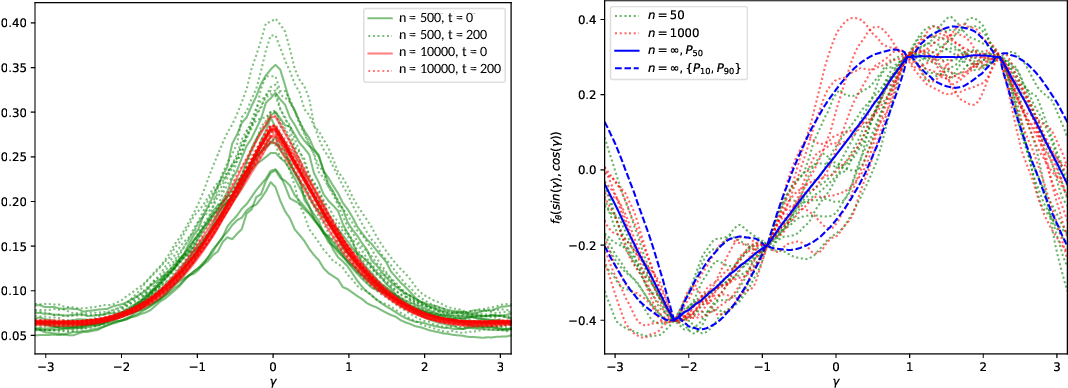
\includegraphics[width=\textwidth]{pic/NTK_paper_exp.png} % Path to the image file
% \caption{} % Caption for the figure
  \end{frame}
 
 
 
 
 
\section{Literature Review}

\begin{frame}{CNTK}
\begin{itemize}
	\item The first efficient exact algorithm for computing the extension of NTK to convolutional neural nets, which we call Convolutional NTK
	\item Theoretically, also
	gives the first non-asymptotic proof showing that a fully-trained sufficiently wide net is indeed equivalent to the kernel regression predictor using NTK.
\end{itemize}
\end{frame}

\begin{frame}{NTK Sketch}
	
	\textbf{Theorem} Given \( x, x' \in \mathbb{R}^d \) and \( \delta \in (0, 1), \epsilon \in (0, 1/L) \), the NTK Sketch computes \( \Phi^{(L)} \in \mathbb{R}^m \), \( m = \mathcal{O}\left(\frac{1}{\epsilon^2} \log \frac{1}{\delta}\right) \) in time
	\[
	\tilde{O}\left( \frac{L^{11}}{\epsilon^{6.7}} + \frac{L^3}{\epsilon^2} d \right)
	\]
	such that
	\[
	\Pr\left[ \left| \left\langle \Phi^{(L)}, \Phi^{(L)'} \right\rangle - K_{\text{NTK}}^{(L)}(x, x') \right| \leq \epsilon \cdot K_{\text{NTK}}^{(L)}(x, x') \right] \geq 1 - \delta.
	\]

\end{frame}



\begin{frame}{Finite Width}
	
They provide quantitative bounds measuring the \(L_
2\) difference in function space between the trajectory of a finite-width network trained on finitely many samples from the idealized kernel dynamics
of infinite width and infinite data.
	
\end{frame}


\begin{frame}{Spectral Bias}
	\begin{itemize}

	\item As an implication of these bounds, eigenfunctions of the NTK integral operator (not just their empirical approximations) are learned at rates corresponding to their eigenvalues
	 
	\item We demonstrate that the network will inherit the bias of the kernel at the beginning of training
	even when the width only grows linearly with the number of samples
	
	\end{itemize}
\end{frame}





\begin{frame}{Generalization Bound}


\begin{itemize}
	\item Assuming:
		\item Fix failure probability \(\delta \in (0,1)\)
		\item data \(S = \{(x_i,y_i)\}_{i=1}^n\)
		\item Distribution \( D \) is \( (\lambda_0, \delta/3, n) \)-non-degenerate.
		\item \( \kappa = \mathcal{O}\left( \frac{\lambda_0 \delta}{n} \right) \).
		\item Width \( m \geq \kappa^{-2} \text{poly}(n, \lambda_0^{-1}, \delta^{-1}) \).
		\item Loss function \( \ell: \mathbb{R} \times \mathbb{R} \to [0, 1] \) is 1-Lipschitz in the first
		argument such that \( \ell(y, y) = 0 \).
		\item Gradient descent runs for \( k \geq \Omega\left( \frac{1}{\eta \lambda_0} \log \frac{n}{\delta} \right) \) iterations.
	

\end{itemize}

\end{frame}



\begin{frame}{Generalization Bound}
	
	
	\begin{itemize}
	\item Then with probability at least  \(1-\delta\) over the random initialization and the training
	samples,The two-layer neural network \(f_{\mathbf{W}(k), \mathbf{a}}\) has population loss \( L_D(f_{\mathbf{W}(k), \mathbf{a}}) = \mathbb{E}_{(\mathbf{x},y)\sim D}[\ell(f_{\mathbf{W}(k), \mathbf{a}}(\mathbf{x}),y)] \), bounded as: 
	
		
		\[
		L_D(f_{\mathbf{W}(k), \mathbf{a}}) \leq \sqrt{\frac{2 \mathbf{y}^\top (\mathbf{H}^\infty)^{-1} \mathbf{y}}{n}} + O\left( \sqrt{\frac{\log \frac{n}{\lambda_0 \delta}}{n}} \right).
		\]
		
	\end{itemize}
	
\end{frame}


\begin{frame}{Uniform Convergence}
	\begin{itemize}
		
\item Overparametrized Multilayer Neural Networks: Uniform Concentration of Neural Tangent Kernel and Convergence of Stochastic Gradient Descent (2024)
\item They first show that with random initialization, the NTK function converges to some
deterministic function uniformly for all layers as the number of neurons tends to infinity
\item Then they apply the uniform convergence result to further prove that the prediction error of multi-layer neural networks under SGD converges in expectation in the streaming data setting
	\end{itemize}

\end{frame}


\begin{frame}{Uniform Convergence}

\textbf{Theorem} Under Gaussian initialization, for \( m \geq C d^2 \exp(L^2) \) for some constant \( C \), there exist constants \( C_1, C_2, \) and \( C_3 \) such that, with probability at least \( 1 - \exp(-C_1 m^{1/3}) \),
\[
\left\| H^{(\ell)} - \Phi^{(\ell)} \right\|_{\infty} \leq C_2 \left( \frac{C_3^L}{m^{1/6}} + \sqrt{\frac{d L \log m}{m}} \right), \quad \forall 1 \leq \ell \leq L.
\]

	
\end{frame}


\section{Proposal}

%\begin{frame}{Related Possible Areas}
%	\item Random Matrix Theory and NTK Spectrum Analysis
%	\item Generalization Bounds Using NTK in High Dimensions
%\end{frame}

\begin{frame}{Our Proposal}
\begin{itemize}
	\item Guarantees with other/practical Assumptions
	\begin{itemize}
		\item NTK-like results on Attention Mechanism
		\item Extending current results on Gaussian/Bounded to sub-Gaussian or sub-Exponential
	\end{itemize}
	\item NTK on Unsupervised settings like Generative modeling or Self-Supervised or Transfer learning
	
	\item NTK on other architectures like Kolmogorov Arnold Networks, Transformers etc

\item  NTK Spectral Distribution
\item Optimization methods other than (Stochastic) Gradient Descent. e.g. Momentum SGD, using Long Search for GD.
\item Certain activation functions. e.g. tanh
\item Random number of neurons in Layers.
\item Finding Sample complexity, VC-Dimensions, Rademacher Complexity
\end{itemize}
\end{frame}


\section{References}

%\begin{frame}{Contributions}
%\textbf{These slides are authored by:}
%    \begin{itemize}
%        \item Hooman Zolfaghari
%    \end{itemize}
%    
%\end{frame}


\begin{frame}[allowframebreaks]
   \bibliographystyle{ieeetr} % Place the style before bibliography
   \bibliography{ref.bib} % Point to your .bib file
   \nocite{*} % Include all references even if not cited
\end{frame}


\end{document}